%%%%%%%%%%%%%%%%%%%%%%%%%%%%%%%%%%%%%%%%%%%%%%%%%%%%%%%%%%%%%%%%%%%%%%%%
\chapter{Fundamentals}
\label{sec:fundamentals}
%%%%%%%%%%%%%%%%%%%%%%%%%%%%%%%%%%%%%%%%%%%%%%%%%%%%%%%%%%%%%%%%%%%%%%%%

In this section multiple solutions for real time collaboration will be analyzed. 
The results from the survey will be used as a basis for the requirements analysis.

%=======================================================================
\section{State of the Art}
\label{sec:stateoftheart}
%=======================================================================

This section describes and discusses current state of the art tools for real time collaboration.

\subsection{Scientific Solutions}

In this section, scientific solutions for real time collaboration will be discussed.

\subsubsection{CoVim}
CoVim\cite{ChoNgSun:2017:CoVim:Incorporatingreal-timecollaborationcapabilitiesintocomprehensivetexteditors} uses Operational Transforms just like Teletype for Atom. But uses a different method of detecting state changes. Instead of observing user interactions it observes changes to files and generates Operational Transforms from diffing states.

\subsubsection{TouchDevelop}
TouchDevelop\footnote{https://www.touchdevelop.com} is an experimental web based editor. It enables real time collaboration by merging ASTs. The paper claims "Indeed, we claim that this approach is generalizable to a
general-purpose language, as long as the editor can parse the
program being edited and transparently tag AST nodes with
an identifier. Naturally, this requires non-trivial support from
the editor".\cite{ProtzenkoBurckhardtMoskalMcClurg:2015:Implementingreal-timecollaborationinTouchDevelopusingASTmerges} The AST translation would have to be implemented for every programming language supported. Additionally the transformation from AST to text might not guarantee the same code just the same AST which could lead to confusion for developers.\autoref{fig:touchdevelop}
\begin{figure}[hb]
    \centering
    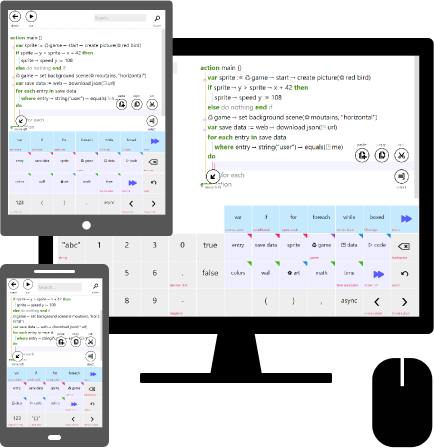
\includegraphics{figures/screenshots/touchdevelop.png}
	\caption{Microsoft TouchDevelop }
	\href{https://www.touchdevelop.com/}{https://www.touchdevelop.com/}
    \label{fig:touchdevelop}
\end{figure}
\subsubsection{CodeR}
CodeR\cite{KurniawanSoesantoWijaya:2015:CodeR:Real-timeCodeEditorApplicationforCollaborativeProgramming} is a Web IDE with built in chat for the programming languages C, C++ and JAVA. 
\begin{figure}[hb]
    \centering
    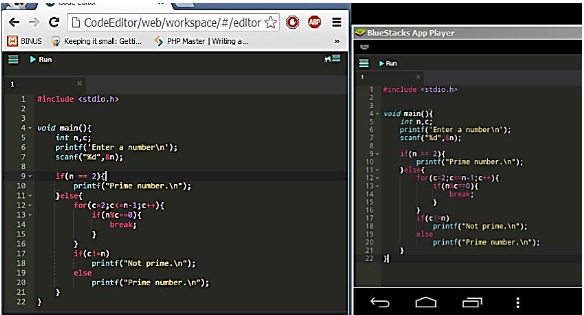
\includegraphics[width=100mm]{figures/screenshots/CodeR.png}
	\caption{CodeR }
	\cite{KurniawanSoesantoWijaya:2015:CodeR:Real-timeCodeEditorApplicationforCollaborativeProgramming}
    \label{fig:touchdevelop}
\end{figure}

\newpage
\subsection{Available Software Tools}

In this section, currently available software solutions for real time collaboration will be discussed.

\subsubsection{Teletype for Atom}
Teletype for Atom\footnote{https://github.com/atom/teletype/issues/211} is a Project enabling editing files peer to peer. It is based on 	\cite{Oster:2006:DataconsistencyforP2Pcollaborativeediting} \cite{YuWeihai:2014} \cite{BriotUrsoShapiro:2016:HighResponsivenessGroupEditing}.
With Teletype it is possible to edit files currently opened by the "host". The files are only persisted on the "host" not on all peers.\footnote{https://teletype.atom.io/}
Therefore disconnecting from the network cuts off the editing workflow. It is not possible to access all the files in a project unless they are opened by the host. 
\subsubsection{Visual Studio Live Share}
Visual Studio Live Share\footnote{https://visualstudio.microsoft.com/de/services/live-share/}  is a plugin for Visual Studio Code and Visual Studio that enables sharing all files of a project loaded in the editor with someone else. In addition to that it enables sharing debugging sessions and ports opened by debugging sessions are forwarded to clients. As with Teletype for Atom files are only persisted on the "host". \autoref{fig:liveshare}
\begin{figure}[hb]
    \centering
    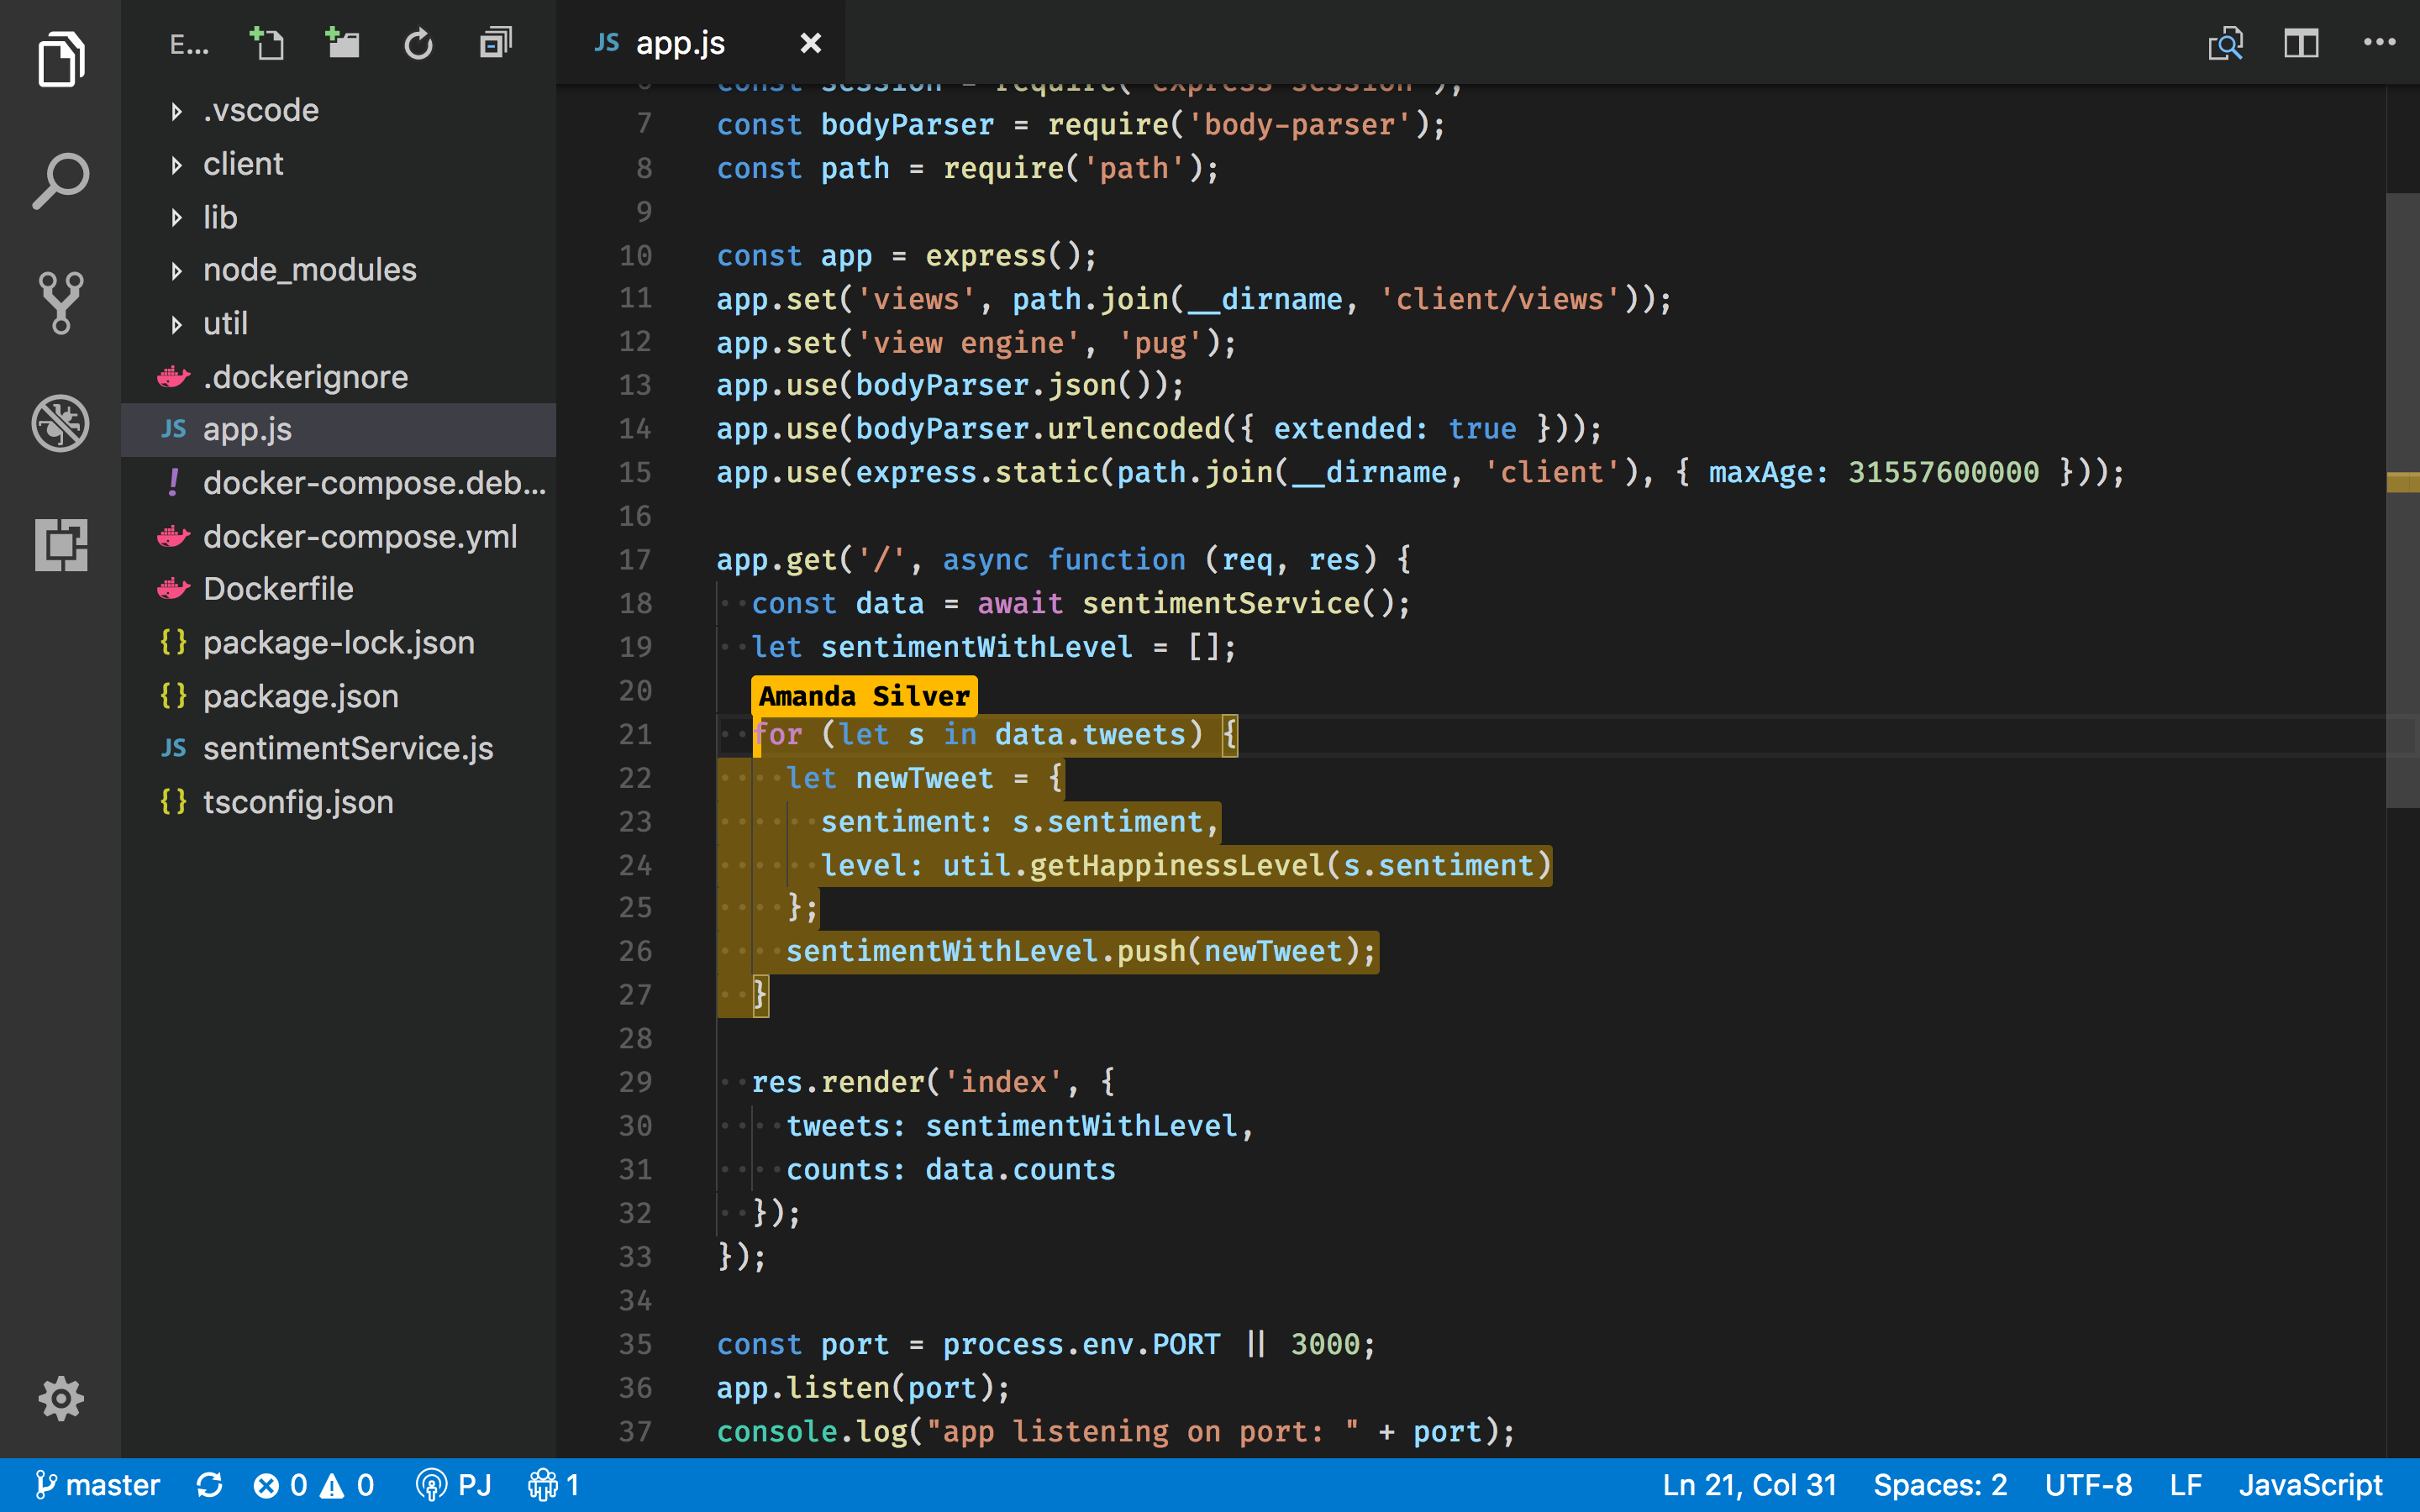
\includegraphics[width=100mm]{figures/screenshots/vscodeliveshare.png}
	\caption{Visual Studio Live Share}
	\href{https://code.visualstudio.com/blogs/2017/11/15/live-share}{https://code.visualstudio.com/blogs/2017/11/15/live-share}
    \label{fig:liveshare}
\end{figure}
\subsubsection{Multihack-Brackets}
Multihack-Brackets\footnote{https://github.com/multihack/multihack-brackets} is a plugin for the Brackets editor. It enables sharing an entire folder structure. It requires a server. As of 13.3.2019 it is not possible to verify performance or functionality since joining a session just crashes the brackets editor. Apparently the development has been stopped. The last commit in the repository was over a year ago (in February of 2018).
\subsubsection{Codeshare}
Codeshare\footnote{https://codeshare.io} is a web based collaborative editor. It is designed for interviews. The editor window offers syntax highlighting for a broad range of programming languages. One shared room always only contains a single file. \autoref{fig:codeshare}
\begin{figure}[h]
    \centering
    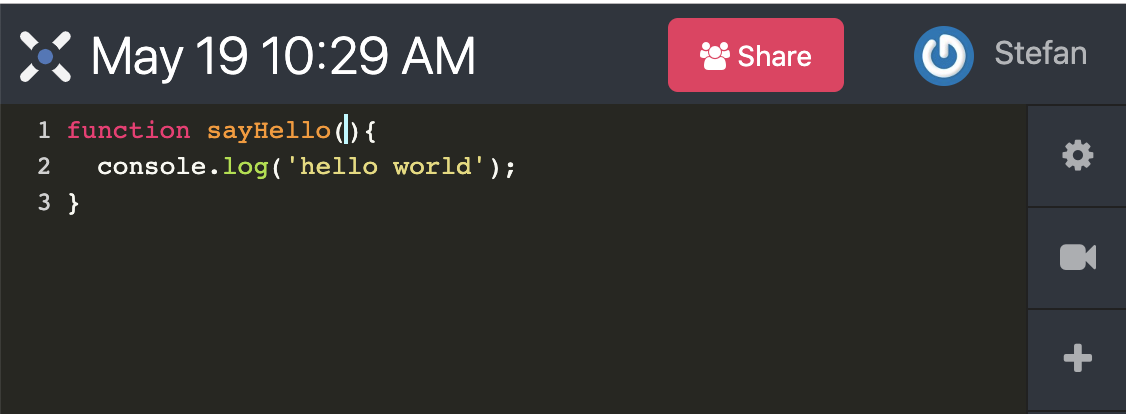
\includegraphics[width=100mm]{figures/screenshots/codeshare.png}
	\caption{Codeshare}
	\href{https://codeshare.io}{https://codeshare.io}
    \label{fig:codeshare}
\end{figure}
\subsubsection{Collabode}
Collabode\cite{Goldman:2011:RCC:2047196.2047215} is "a web-based Java integrated development environment". It shares changes between developers as soon as they have no compilation errors. It is designed for the Java language. (See \autoref{fig:collabode})
\begin{figure}[h]
    \centering
    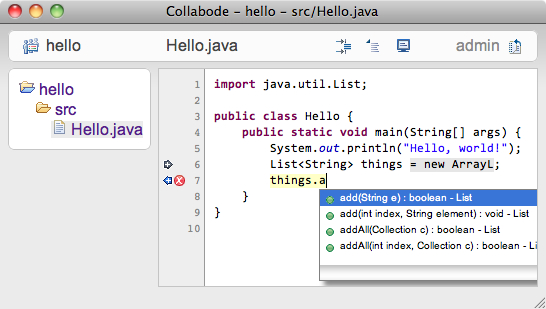
\includegraphics[width=100mm]{figures/screenshots/collabode.jpg}
	\caption{Collabode}
	\cite{Goldman:2011:RCC:2047196.2047215}
    \label{fig:collabode}
\end{figure}
\subsection{Summary}
As described in \autoref{tab:sota} current solutions are mostly implemented as extensions to code editors. Only codeshare is web based because it is based around the use-case of doing interviews. Overall none of the current solutions have any considerations for dealing with an underlying version control system of a project.

\begin{table}
	\centering
	\begin{tabular}{| >{\bfseries}l | l | l | l | l | }
		\hline
			\rowcolor{orange} \bfseries Tool & \bfseries Type & \bfseries Location & \bfseries Shared Content \\
		\hline
		\hline
			Teletype for Atom & Extension & Host & Individual Files \\\hline
			Visual Studio Live Share & Extension & Host & Project Folder \\\hline
			Multihack Brackets & Extension &  Distributed? & Project Folder \\\hline
			Codeshare & Web application & Server & Single File \\\hline
			Collabode & Web application & Server & Project Folder \\\hline
			TouchDevelop & Web application & Server & Entire Project \\
		\hline
	\end{tabular}
	\caption{Overview state of the art}
	\label{tab:sota}
\end{table}

\section{CRDT}
In order to update shared objects stored at different sites a "commutative replicated data type" or CRDT is proposed by \cite{PreguicaMarquesShapiroLetia:2009}. The idea is to design the underlying representation or data structure of edits to a document such that operations are commutative and therefore automatically converge at every copy of the document.
But there is a problem with this approach. If there are concurrent insertions at the same position of a document, a global order for the conflicting information has to be established. \cite{PreguicaMarquesShapiroLetia:2009},\cite{Oster:2006:DataconsistencyforP2Pcollaborativeediting} have a solution to this problem: every site gets a unique siteID and a logical clock or counter. Concurrent inserts are then ordered either by the counter (smaller counter first) or if the counters are identical by the siteID.

\section{Scrum}
Scrum is an agile, iterative software development process. Work is divided into Sprints. There are daily meetings called "Daily Scrum". In those meetings important questions are evalutated as a group. One of them is "What impediments stand in the way of you meeting your commitments to this Sprint and this project?".\cite{schwaber2004agile},\cite{10.1007/978-1-4471-0947-1_11}
In theory this introduces a maximum delay of one day from potentially blocking code being written to the person depending on it knowing about it. This time can further be decreased by establishing tighter communication between team members.
Especially in distributed development, it is important to "Arrange an access to multiple communication tools"\cite{5196933} for unofficial distributed meetings.\cite{4638656}
Since the version control system is a communication tool, improving version control systems improves communication tools and aids Scrum based software development processes.

\section{Code Review}

Companies like Google and Microsoft use a process called "code review" to validate changes. The basic idea is that before merging a code modification onto master, it is reviewed by someone else. This keeps code quality stable and educates developers.\cite{SadowskiSoederbergChurchSipkoBacchelli:2018:Moderncodereview:acasestudyatgoogle},\cite{Bacchelli:2013:EOC:2486788.2486882},\cite{7081824} This thesis aims to support these workflows while enhancing the developer experience. 

"Another thing we focused on was performance. For that
reason, even today CodeFlow remains a tool that works
client-side, meaning you can download your change first
and then interact with it, which makes switching between
files and different regions very, very fast."\cite{CzerwonkaGreilerBirdPanjerCoatta:2018:CodeFlow:ImprovingtheCodeReviewProcessatMicrosoft} Therefore another important goal for this thesis is to deliver an experience that works client side and keeps working when disconnecting and reconnecting to networks.